\documentclass[12pt,a4paper]{report}

\usepackage{setspace}
\renewcommand{\baselinestretch}{1.2}

\usepackage[round]{natbib}
\usepackage{epsfig}
\usepackage{amsmath,amsfonts,amsthm,amssymb}
\usepackage{setspace}
\usepackage{fancyhdr}
\usepackage{lastpage}
\usepackage{extramarks}
\usepackage{chngpage}
\usepackage{soul}
\usepackage[top=1in, bottom=1in, right=1in, left=1.5in]{geometry}
\usepackage{enumerate}
\usepackage[usenames,dvipsnames]{color}
\usepackage{graphicx,float,wrapfig}
\usepackage{ifthen}
\usepackage{courier}
\usepackage{listings}

\DeclareMathOperator*{\argmin}{\arg\!\min}
\renewcommand\bibname{References}
\definecolor{MyDarkGreen}{rgb}{0.0,0.4,0.0}

\lstloadlanguages{R}%
\lstset{
    language=R,
    frame=single,
    basicstyle=\small\ttfamily,
    keywordstyle=[1]\color{Blue}\bf,
    keywordstyle=[2]\color{Purple},
    keywordstyle=[3]\color{Blue}\underbar,
    identifierstyle=,
    commentstyle=\usefont{T1}{pcr}{m}{sl}\color{MyDarkGreen}\small,
    stringstyle=\color{Purple},
    showstringspaces=false,
    tabsize=5,
    % Put standard R functions not included in the default
    % language here
    morekeywords={rq, qplot, geom, abline, show, guide, aes, brq, lqm, TRUE, FALSE, bayesQR},
    % Put R function parameters here
    morekeywords=[2]{on, off, interp},
    % Put user defined functions here
    morekeywords=[3]{FindESS},
    morecomment=[l][\color{Blue}]{...},
    numbers=left,
    firstnumber=1,
    numberstyle=\tiny\color{Blue},
    stepnumber=5
}

\begin{document}
\begin{titlepage}
\vspace*{\fill}
\begin{center}
\Huge{\textbf{Quantile Regression}}\\
\Large{Reference range of Thyroid function test in pregnancy}\\
\vspace{5mm}
\Large{\textbf{Kevin Brosnan}}\\
\vspace{5mm}
\Large{Final Year Project: Interim Report}\\
\Large{Mathematical Sciences}\\
\vspace{5mm}
\begin{figure}[h]
\begin{center}

\includegraphics{ullogo.jpg}
\end{center}
\end{figure}
\Large{Department Of Mathematics and Statistics}\\
\Large{University of Limerick}\\
\Large{Limerick}\\
\Large{Ireland}\\
\Large{November, 2013}\\
\vspace{10mm}
\large{A final year project submitted in partial fulfillment of the B.Sc degree in Mathematical Sciences}\\
\vspace{6mm}
\Large{Supervisor: Dr. Kevin Hayes}\\
\Large{Second Reader: Dr. Norma Bargary}
\end{center}
\vspace*{\fill}
\end{titlepage}

\pagenumbering{roman}

\chapter*{Abstract}


\chapter*{Acknowledgements}
I wish to thank the academic staff of the Maths and Statistics Department of University of Limerick for all the knowledge they have instilled on me over the course of my undergraduate programme. I would like to express my deep gratitude to Dr. Kevin Hayes, my supervisor, for his patient guidance, enthusiastic encouragement and useful critiques of my final year project.
\vspace{2mm}
\par\noindent
Finally, I wish to thank my parents for their support and encouragement throughout my study.

\tableofcontents

\clearpage
\pagenumbering{arabic}
\chapter{Introduction}
Thyroid disorders are the second most common endocrinologic disorders found in pregnancy. Overt hypothyroidism is estimated to occur in $0.3-0.5\%$ of pregnancies. Subclinical hypothyroidism tends to occur in $2-3\%$, and hyperthyroidism is present in $0.1-0.4\%$.\citep{Thyroid-Facts} Physiological changes of pregnancy, including $50\%$ increase in plasma volume, increased thyroid binding globulin production and a relative iodine deficiency, means that thyroid hormone reference ranges for non-pregnant women may not be appropriate in pregnancy.
\vspace{2mm}

One acceptable approach for establishing legitimate reference ranges requires that a Box-Cox transformation be applied to the data and prediction ranges calculated using classical polynomial regression. Alternatively, non-parametric smoothing such as quantile regression can be used to estimate the $2.5\%$ and $97.5\%$ percentiles. While this approach provides an estimate of the reference range, there are problems with the method. The main problem is the issue of crossing quantiles which makes it difficult to assign each patient to a single range. This is the issue that will be focused on throughout this project.

\chapter{Analytical Background}
The objective of regression analysis is to establish a relationship between a response variable, $Y$, and the predictor variables, $\{x_{1},\ldots,x_{p}\}$. In real world applications, $Y$ cannot be calculated perfectly from the $X$ variables. For modelling purposes we formulate $Y$, for a fixed value of each $x_{i}$ as a random variable. We generally proceed by summarising the relationship of the response variable for fixed values of the predictors using measures of centrality, specifically the mean, median and mode.
\vspace{2mm}

Quantile regression uses the median as its central tendency and is the method of interest in this project. In this chapter we outline the theory behind quantile regression, focusing attention on the frequentist approach to quantile regression, Bayesian quantile regression and linear quantiles for mixed models. Finally, we will examine the computational implementation required for each of the quantile regression methods outlined above.

\section{Quantiles}
A quantile $\tau$ of the dependant variable $Y$ is defined such that $100\tau\%$ of the population have values less than the $\tau^{th}$ quantile and $100(1-\tau)\%$ of the population have values greater than the $\tau^{th}$ quantile (see Figure \ref{Graph:Quantile}).
\vspace{2mm}

\begin{figure}[ht]\centering
    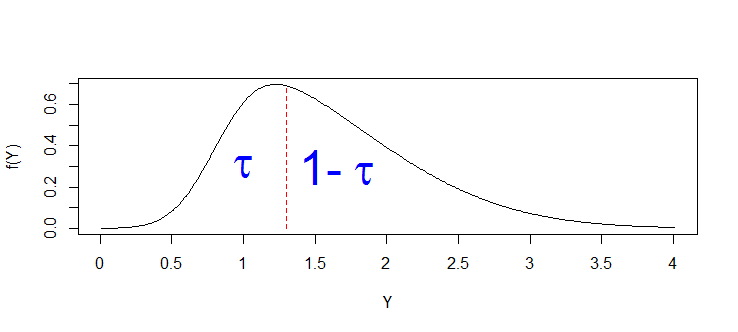
\includegraphics[width=10cm]{Quantiles.png}
    \caption{Graphical illustration of the $\tau^{th}$ quantile.}
    \label{Graph:Quantile}
\end{figure}

The median is defined such that 50\% of your population have a value above this value and 50\% of your population have a value below this value. The median can therefore be interrupted as the $0.5^{th}$ quantile. The quantile or percentile refers to the general case of this.
\vspace{2mm}

More formally, let $Y$ be a continuous real valued random variable, it may be characterised by its distribution function as
    $$F_{Y}(y)=\mathbb{P}(Y \leq y),$$
while for any $0 < \tau <1$,
    $$ Q(\tau) = \inf\left\{y : F_{Y}(y) \geq \tau\right\}$$
is called the $\tau^{th}$ quantile of $Y$. When estimating quantiles, we want to determine the value of $y$ in the sample data corresponding to a given probability $\tau$. The $\tau^{th}$ quantile in a sample of data refers to the probability of $\tau$ for a value $y$, such that
    $$F_{Y}(y_{\tau})=\tau.$$
Another form of expressing the $\tau^{th}$ quantile mathematically is
    $$y_{\tau}=F^{-1}_{Y}(\tau).$$
$y_{\tau}$ is such that it constitutes the inverse of the function $F_{Y}(\tau)$ for a probability $\tau$.
\vspace{2mm}

If the distribution function $F_{Y}(y)$ is monotonically increasing, quantiles are well defined for every $\tau \in (0,1)$. However, if a distribution function $F_{Y}(y)$ is not strictly monotonically increasing, there are some $\tau$'s for which a unique quantile can not be defined. In the latter case one must use the smallest value that $y$ can take on for a given probability $\tau$. In both cases the problem can be defined mathematically as seeking the value of $y$ satisfying
\begin{equation}
\label{eq:Quantiles}
    y_{\tau}=F^{-1}_{Y}(\tau)=\inf\left\{y:F_{Y}(y)\geq\tau\right\}.
\end{equation}
\vspace{2mm}
Therefore, $y_{\tau}$ is equal to the inverse of the function $F_{Y}(\tau)$ which in turn is equal to the infimum of $y$ such that the distribution function $F_{Y}(y)$ is greater or equal to a given probability $\tau$ which in turn is the $\tau^{th}$ quantile.

\section{Quantile Regression}
Quantile regression is a statistical technique used to estimate conditional quantile functions. Classic linear regression methods are based on minimising sum-of-squares residuals and can be used to estimate models for conditional mean functions. Quantile regression methods however offer a way of estimating models for the conditional median function and all other conditional quantile functions. As quantile regression can estimate the entire family of
conditional quantile functions it provides a much more powerful statistical analysis of relationships among random variables \citep{QR-Intro}. The need for something beyond linear regression was first advocated by \citet{Motivation}:
\vspace{2mm}

\par \noindent
{\textit{What the regression curve does is give a grand summary for the averages of the distributions corresponding to the set of of x's. We could go further and compute several different regression curves corresponding to the various percentage points of the distributions and thus get a more complete picture of the set. Ordinarily this is not done, and so regression often gives a rather incomplete picture. Just as the mean gives an incomplete picture of a single distribution, so the regression curve gives a correspondingly incomplete picture for a set of distributions.} \citep{Motivation}}
\vspace{2mm}

\begin{flushleft}
Features that characterise quantile regression and distinguish it from other regression methods are the following:
\end{flushleft}
\begin{enumerate}
    \item quantile regression can characterise the entire conditional distribution of $Y$ through different values of $\tau$;
    \item heteroscedasticity can be detected;
    \item median regression estimators can be more efficient then mean regression estimators if heteroscedasticity is detected;
    \item the minimisation problem as illustrated in equation \ref{eq:QR-min} can be solved efficiently by linear programming methods, making estimation easy;
    \item quantiles are robust in regards to outliers.
\end{enumerate}

The technical details in the remainder of this section will help to explain how to implement quantile regression contrasting three fitting methods. Quantile regression can be seen as one statistical method which can be used to complete the regression picture.

\subsection{Frequentist Approach}
Quantile regression transforms a conditional distribution function into a conditional quantile function by slicing it in to segments. These segments describe the cumulative distribution of a conditional variable $Y$ given the explanatory variables $x_{i}$ with the use of quantiles as defined in equation (\ref{eq:Quantiles}). For a dependant variable $Y$ given the explanatory variable $X=x$ and fixed $\tau$, $0<\tau<1$, the conditional quantile function is defined as the $\tau^{th}$ quantile $Q_{Y|X}(\tau|x)$ of the conditional distribution function $F_{Y|X}(y|x)$. For the estimation of the location of the conditional distribution function, the conditional median $Q_{Y|X}(0.5|x)$ can be used as an alternative to the conditional mean.
\vspace{2mm}

In ordinary least squares, modelling a conditional distribution function of a random sample $(y_{1},\ldots,y_{n})$ with a parametric function $\mu(x_{i},\beta)$ where $x_{i}$ represents the independent variables, $\beta$ the corresponding estimates and $\mu$ the conditional mean, one addresses the minimisation problem
    $$\min_{\beta\in\Re}\sum^{n}_{i=1}(y_{i}-\mu(x_{i},\beta))^{2}.$$
We therefore obtain the conditional expectation function $\mathbb{E}[Y|x_{i}]$. The conditional expectation function is the best predictor of $Y$ given $x_{i}$ in the sense that it solves a minimum mean squared error prediction problem. It can be simply evaluated as
$$ \mathbb{E}[Y|x_{i}]=\argmin_{m(x_{i})}\mathbb{E}[(Y-m(x_{i}))^2] $$
where $m(x_{i})$ is any function of $x_{i}$. This equation is minimised at $m(x_{i}) = \mathbb{E}[Y|x_{i}]$. While the approach is similar for quantile regression the central feature now becomes $\rho_{\tau}$, which acts as a check function. Define $\rho_{\tau}(x)$ by
    \[
        \rho_{\tau}(x)=
        \begin{cases}
        \tau*x,& \text{if } x\geq0\\
        (\tau-1)*x,& \text{if } x<0
        \end{cases}
    \]

\begin{figure}[ht]\centering
    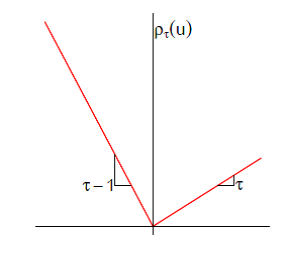
\includegraphics[width=7cm]{CheckFunctionImage.png}
    \caption{Quantile Regression $\rho$ Function}
\end{figure}
\vspace{2mm}

The check function, $\rho_{\tau}(x)$, ensures that:
\begin{enumerate}[(i)]
    \item all $\rho_{\tau}$ are positive;
    \item the scale is according to the probability $\tau$.
\end{enumerate}

In quantile regression, the $\tau^{th}$ \textit{sample} quantile may be found by solving:
\begin{equation}
\label{eq:QR-min}
    \min_{\xi\in\Re}\sum^{n}_{i=1}\rho_{\tau}(y_{i}-\xi)
\end{equation}
While it is more common to define the sample quantiles in terms of the order statistics, $y_{(1)}\leq y_{(2)} \leq \ldots \leq y_{(n))}$, which results in a sorted arrangement of the original sample. Their formulation as a minimisation problem has the advantage that it yields a natural generalisation of the quantiles to the regression context.
The idea of estimating the unconditional mean is simply
$$ \hat{\mu}=\argmin_{\mu\in\Re}\sum(y_{i}-\mu)^{2}.$$
This estimation can be extended to the estimation of the linear conditional mean function $E(Y|X=x)=x'\beta$ by solving
$$ \hat{\beta}=\argmin_{\beta\in\Re^{p}}\sum(y_{i}-x'\beta)^2.$$
Similarly, the linear conditional quantile function, $Q_{Y}(\tau|X=x)=x_{i}'\beta(\tau)$, can be estimated by solving the minimiser
$$ \hat{\beta}=\argmin_{\beta\in\Re^{p}}\sum\rho_{\tau}(y_{i}-x'\beta).$$
In contrast to ordinary least squares, the minimisation in quantile regression is done for each subset defined by $\rho_{\tau}$. The $\tau^{th}$ quantile is estimated with the parametric function $\xi(x_{i},\beta)$. The requirement for the square in the unconditional mean case is to ensure each calculated term is positive, the check function $\rho_{\tau}$ ensures this in the quantile regression case and so the square of difference is not required.

\subsection{Bayesian Approach}
Unlike the frequentist approach to statistics, the Bayesian approach provides us with the entire posterior distribution of the parameter of interest. Additionally, it allows for uncertainty of a parameter to be taken into account when making a prediction. Irrespective of the true distribution of the data, Bayesian inference for quantile regression produces the likelihood function based on the asymmetric Laplace distribution.
\vspace{2mm}

A random variable $\omega$ follows the asymmetric Laplace distribution if its probability density function is given by
$$ f_{\tau}(\omega; \mu,\sigma) = \frac{\tau(1-\tau)}{\sigma}\exp\left\{-\rho_{\tau}\left(\frac{\omega-\mu}{\sigma}\right)\right\}, $$
where $0<\tau<1$, $\mu$ is the location parameter, $\sigma$ is the scale parameter and $\rho_{\tau}(u)$ is the loss function defined as
    \[
        \rho_{\tau}(x)=
        \begin{cases}
        \tau*x,& \text{if } x\geq0\\
        (\tau-1)*x,& \text{if } x<0,
        \end{cases}
    \]
or in a simpler form,
\begin{equation}
\label{eq:Bay-QR}
\rho_{\tau}(u)=\frac{|u|+(2\tau-1)u}{2}.
\end{equation}
\vspace{2mm}

Using general modelling techniques like ordinary least squares the estimates of the regression parameters $\beta$ are computed by assuming that
\begin{enumerate}[(i)]
    \item conditional on $x$, the random variables $Y_{i}$, are mutually independent with distributions $f(y;\mu_{i})$ specified by the values of $\mu_{i}=E[Y_{i}|x_{i}]$;
    \item for some known link function $g$, $g(u_{i})=x_{i}'\beta$.
\end{enumerate}

However, in this project we are interested in the conditional quantile, $q_{\tau}(y_{i}|x_{i})$, in contrast to the conditional mean, $E[Y_{i}|x_{i}]$. Simple assumptions can be made so that regardless of the distribution of the data it is possible to solve for the quantiles in the framework of the general linear model. Assuming the following makes this possible,
\begin{enumerate}[(i)]
    \item $f(y; \mu_{i})$ is asymmetric Laplace;
    \item $g(\mu_{i})=x_{i}'\beta(\tau)=q_{\tau}(y_{i}|x_{i})$ for any $0<\tau<1$.
\end{enumerate}

An issue with using Bayesian statistics is the requirement of a conjugate prior distribution for quantile regression formulation. While this is generally not known Markov Chain Monte Carlo (MCMC) methods can extract posterior distributions of the unknown parameters which allows the use of any prior distribution. While giving us the marginal and joint posterior distributions of all the unknown parameters, the Bayesian approach, also provides us with a very practical way of including parameter uncertainty in predictive inferences.
Given the observations, $y=(y_{1},\ldots,y_{n})$, the posterior distribution of $\beta$, $\pi(\beta|y)$ is given by
$$\pi(\beta|y) \propto L(y| \beta) p( \beta),$$
where $p(\beta)$ is the prior distribution of $\beta$ and $L(y|\beta)$ is the likelihood function written as
\begin{equation}
\label{eq:Bay-Likelihood}
    L(y|\beta)=\tau^{n}(1-\tau)^{n}\exp\left\{-\sum_{i}\rho_{\tau}(y_{i}-x_{i}'\beta)\right\}
\end{equation}
which is using equation \ref{eq:Bay-QR} with a location parameter $\mu_{i}=x_{i}'\beta$.
\vspace{2mm}

The optimum strategy is to choose $\beta$ such that the resulting joint posterior distribution will be proper. It can be shown that the best choice for the prior of $\beta$ is for it to be improper uniform.

\subsection{Linear Mixed Models Approach}
In statistics it is sometimes necessary to take into account the correlation of observations which belong to the same unit or cluster of the data being analysed. Mixed effects models represent an efficient, flexible and popular way of analysing this complex data. The modelling technique attempts to model and estimate the variability between clusters by using cluster specific random effects. The fact that mixed models can estimate the between cluster variability is a significant advantage over standard modelling techniques as they can provide conditional inferences. In mixed models, both fixed and random effects are assumed to be location-shift effects.
\vspace{2mm}

The general idea of linear mixed models approach for quantile regression came from Marco Geraci and Matteo Bottai's asymmetric Laplace approach. A generalisation of this model was further developed by \citet{lqmm} and is the foundation of the {\small\verb"lqmm R"} package which will be discussed later.
\vspace{2mm}

A continuous random variable $\omega\in\Re$ is said to follow an asymmetric Laplace distribution with parameters $(\mu,\sigma,\tau)$, $\omega\sim AL(\mu,\sigma,\tau)$, if its density can be expressed as
$$ p(\omega|\mu,\sigma,\tau)=\frac{\tau(1-\tau)}{\sigma}\exp\left\{-\frac{1}{\sigma}\rho_{\tau}(\omega-\mu)\right\} $$
\vspace{1.5mm}
where $-\infty<\mu<\infty$ is the location parameter, $\sigma >0$ is the scale parameter, $0<\tau<1$ is the skew parameter and $\rho_{\tau}(\upsilon)$ is
    \[
        \rho_{\tau}(x)=
        \begin{cases}
        \tau*x,& \text{if } x\geq0\\
        (\tau-1)*x,& \text{if } x<0
        \end{cases}
    \]
This is the general loss function which is used in each method of quantile regression described in this chapter. In our case, the parameter $\mu$ is of great interest as this is the $\tau^{th}$ quantile of $\omega$, that is that $Pr(\omega\leq\mu)=\tau$.
\vspace{2mm}

If the random variable $\omega$ is comprised of $n$ independent $\omega_{i}'s$ with common skew ($\tau$) and scale ($\sigma$) parameters and different location ($\mu$), then $\omega_{i}\sim AL(\mu_{i},\sigma,\tau)$ for $i={1,\ldots,n}$. This leads to a simplified expression for $\omega's$ density function
$$p(\omega|\mu,\sigma,\tau)=\sigma_{n}(\tau)\exp\left\{-\frac{1}{\sigma}\rho_{\tau}(\omega-\mu)\right\} $$
where $\sigma_{n}(\tau)=\frac{\tau^{n}(1-\tau)^{n}}{\sigma^{n}}$ and $\rho_{\tau}(y-\mu)=\sum_{i=1}^{n}\rho_{\tau}(\omega_{i}-\mu_{i})$.
\vspace{2mm}

\citet{lqmm} proposed a random-intercepts quantile regression model for longitudinal data using the asymmetric Laplace to model the $\tau^{th}$ conditional quantile of a continuous response variable. In particular, they assumed the following regression function
$$ Q_{y|u}(\tau|x,u)=X\beta^{(\tau)} + u,$$
where $(y,X)$ represents the longitudinal data, $u$ a vector of subject-specific random effects and $Q_{y|u}$ denotes the inverse of the unknown distribution $F_{y|u}$. The $\tau^{th}$ regression quantile of $y|u$ was then estimated under the convenient assumption $y|u\sim AL(X\beta^{(\tau)}+u,\sigma^{(\tau)}, \tau)$, where the $\tau$-dependant parameters $\beta^{(\tau)}$ and $\sigma^{(\tau)}$ have a frequentist interpretation. There exists a link between the $L_{1}$ norm regression problem and the asymmetric Laplace based estimation of the coefficients $\beta^{(\tau)}$ which I will not get into here.

\newpage
\section{Implementation}
As {\small\verb"R"} \citep{R} will be used as the development environment for the solution to this problem, we will review the current packages that implement the above quantile regression methods. The main package available in {\small\verb"R"} for each of the methods described above are outlined in the list below. We will discuss each of these methods in the following pages. Advantages, disadvantages and inadequacies of each of the approaches will be highlighted. Included in the following is output from {\small\verb"R"} using the specified approach to compute the quantiles. The sample data used is the Engel data set which is available with the {\small\verb"quantreg"} package available on CRAN. The data consists of income and food expenditure values for $235$ Belgian working class households.

\begin{itemize}
    \item The frequentist method is available in the {\small\verb"quantreg"} package developed by \citet{R-quantreg}
    \item The Bayesian method is available in the {\small\verb"bayesQR"} package developed by \citet{R-bayesQR}
    \item The linear mixed models method is available in the {\small\verb"lqmm"} package developed by \citet{R-lqmm}
\end{itemize}

\subsection{Frequentist Approach}
The frequentist approach to quantile regression is implemented in {\small\verb"R"} through Roger Koenker's extensive {\small\verb"quantreg"} package. The package is currently in version $5.05$. The package contains an array of functions for calculating regression quantiles, plotting the results, formatting the results table and a multitude of data sets which can be used as test data for the package. The basic fitting routine is used as follows {\small\verb"rq(formula, tau=.5, data, method='br')"}. The function can accept more parameters than shown here however these are the parameters of interest here. The {\small\verb"formula"} argument specifies the model that is desired. In the Engel data example below I fitted a simple bivariate linear model so the formula was simply {\small\verb"foodexp~income"}, if we had two explanatory variables it would simply be {\small\verb"foodexp~income + something else"}. The parameter {\small\verb"tau"} is defaulted to calculate the median regression line, however it will accept a single quantile of interest or a vector of quantiles which is used in the example below. The {\small\verb"data"} argument requires the name of the {\small\verb"data.frame"} which contains the variables named in the {\small\verb"formula"} argument. In the case of our example {\small\verb"data=engel"} was passed to the function. The {\small\verb"method"} argument specifies the calculation method which the package should use to calculate the regression quantiles of interest.
\vspace{2mm}

The {\small\verb"rq"} function will automatically use {\small\verb"method='br'"} if no method is specified. The {\small\verb"br"} method calculates the regression quantiles using exterior point methods. It controls the quantile regression fitting by the simplex approach embodied in the algorithm of \citet{KdO1987} based on the median regression algorithm of \citet{BR1974}. If all values of {\small\verb"tau"} lie in $(0,1)$ then the regression values are returned for the single or multiple quantiles requested. On the other hand, if {\small\verb"tau"} lies outside $[0,1]$ parametric programming methods are used to find all the solutions to the quantile regression problem for {\small\verb"tau"} in $(0,1)$. This method is efficient for problems containing up to several thousand observations and has the advantage of being able to calculate the full quantile regression process. It also implements a scheme for computing confidence intervals for the estimated parameters based on an inversion of a rank test described in \citet{RK1994}.
\vspace{2mm}

Two other methods to compute the regression quantiles are {\small\verb"method='fn'"} and {\small\verb"method='pfn'"}. These methods both use the Frisch-Newton algorithm to compute the regression quantiles. The algorithms full detail's are explained in \citet{Frisch-Newton}. In brief, the approach is the reverse of the simplex method, rather than travelling around the exterior of the constraint set it starts from within the constraint set and moves towards the exterior. Instead of taking steepest decent steps at each intersection of exterior edges, it takes Newton steps based on a log-barrier Lagrangian form of the objective function. For exceptionally large problems {\small\verb"method='pfn'"} further adds a pre-processing step to the algorithm which can help to speed up the process considerably.
\vspace{2mm}

There are also two methods for penalised quantile regression available in the package are {\small\verb"method='lasso'"} and {\small\verb"method='scad'"}. These methods implement the lasso penalty and Fan and Li's smoothly clipped absolute deviation penalty, respectively. A parameter {\small\verb"lambda"} is passed to both functions and is key to the calculations made. In the {\small\verb"lasso"} case, if {\small\verb"lambda"} is a scalar quantity the penalty function is the l1 norm of the last coefficients, under the assumption that the first coefficient is an intercept parameter that should not be subject to the penalty. When {\small\verb"lambda"} is a vector it defines a coordinatewise specific vector of lasso penalty parameters. Similarly, for the {\small\verb"scad"} method, if {\small\verb"lambda"} is a scalar quantity the penalty function is the scad modified l1 norm of the last coefficients, under the assumption that the first coefficient is an intercept parameter that should not be subject to the penalty. When {\small\verb"lambda"} is a vector it defines a coordinatewise specific vector of scad penalty parameters. It should be noted that while these methods are available, Koenker himself states that ``These methods should probably be regarded as experimental".
\vspace{2mm}

% Plot of Engel data with Quantile lines
\begin{figure}[ht]\centering
    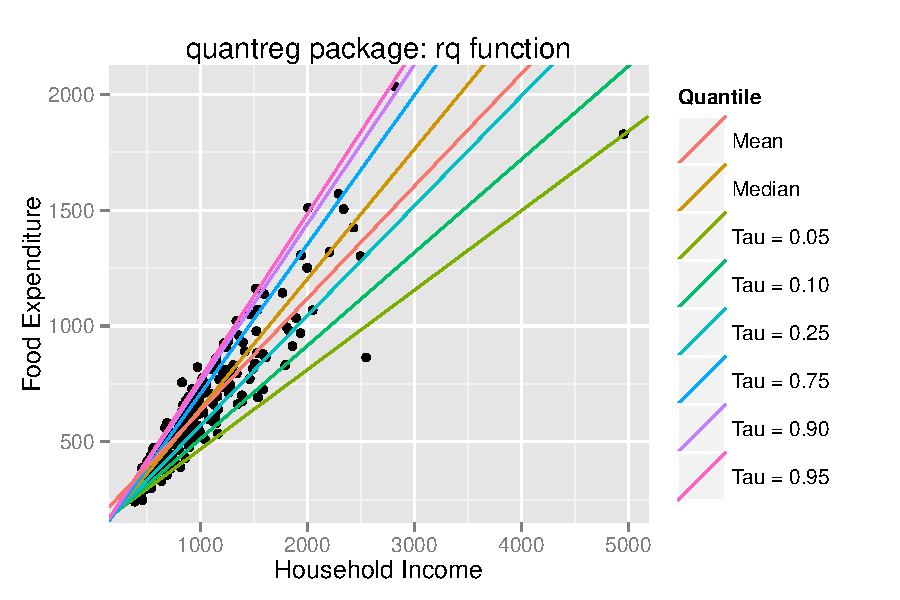
\includegraphics[width=10cm, height=7cm]{PlotofQuantreg.pdf}
    \caption{Quantreg Estimation of Quantiles on Engel Data}
    \label{plot:quantreg-example}
\end{figure}

To provide a somewhat more visual explanation of the {\small\verb"quantreg"} package I will illustrate an example of its usage on the Engel data set available with the package. The data contains $235$ observations of food expenditure and household income for $19^{th}$ century working class Belgian households. Figure \ref{plot:quantreg-example} shows the $\{0.05_{th},0.10_{th},0.25_{th},0.75_{th},0.90_{th},0.95_{th}\}$ quantile regression lines, the median fit and the least squares estimate of the conditional mean function. The quantiles were calculated using the {\small\verb"br"} method as described above. The least squares estimate was computed using the {\small\verb"lm"} function available in {\small\verb"R"} for linear regression. It can be seen at the bottom left of the graph the regression lines intersect with one another which is the issue I hope to address in this paper.
\vspace{2mm}

% Table of Results
\begin{table}[ht]
\begin{center}
\begin{tabular}{|l||c|c|} \hline
\multicolumn{1}{|l||}{Quantile}&\multicolumn{1}{c|}{Intercept}&\multicolumn{1}{c|}{Slope}\tabularnewline
\hline
$\tau$ = 0.05&$\underset{(~98.302,130.517)}{124.880}$&$\underset{(~~0.343,~~0.390)}{~~0.343}$\tabularnewline
$\tau$ = 0.10&$\underset{(~79.888,146.189)}{110.142}$&$\underset{(~~0.342,~~0.451)}{~~0.402}$\tabularnewline
$\tau$ = 0.25&$\underset{(~73.786,120.098)}{~95.484}$&$\underset{(~~0.420,~~0.494)}{~~0.474}$\tabularnewline
Median&$\underset{(~53.259,114.012)}{~81.482}$&$\underset{(~~0.487,~~0.602)}{~~0.560}$\tabularnewline
$\tau$ = 0.75&$\underset{(~32.745,107.314)}{~62.397}$&$\underset{(~~0.580,~~0.690)}{~~0.644}$\tabularnewline
$\tau$ = 0.90&$\underset{(~37.118,103.174)}{~67.351}$&$\underset{(~~0.649,~~0.742)}{~~0.686}$\tabularnewline
$\tau$ = 0.95&$\underset{(~46.265,~83.579)}{~64.104}$&$\underset{(~~0.674,~~0.734)}{~~0.709}$\tabularnewline
Mean&$147.4754$&$~~0.4852$\tabularnewline
\hline
\end{tabular}
\end{center}
\caption{Regression line coefficients for figure \ref{plot:quantreg-example}}
\label{table:quantreg-example}
\end{table}

The quantiles were also calculated after taking a log transformation of the data. This was used as an attempt to stop the quantiles crossing. It can be seen in figure \ref{plot:quantreglog-example} that the quantiles are not crossing at a point close to the origin, however the $0.95^{th}$ and $0.90^{th}$ quantile lines are still crossing. A log transformation therefore does not appear to solve the crossing quantiles problem but does improve on the previous example. The {\small\verb"R"} code used to produce this graphic is available in appendix \ref{App:Engel-Code-Quantreg}.

% Plot of log of Engel data with Quantile lines
\begin{figure}[ht]\centering
    \includegraphics[width=10cm]{PlotofQuantregLog.pdf}
    \caption{Quantreg Estimation of Quantiles on log transformation of Engel Data}
    \label{plot:quantreglog-example}
\end{figure}

Finally, the coefficients of the quantile regression calculations for figure \ref{plot:quantreg-example} are shown in table \ref{table:quantreg-example} while the log transformation coefficients are shown in table \ref{table:quantreglog-example}. The values in parenthesis below the actual value are the confidence bands for that value. Note that the intercept and the slope differ for each of the quantiles and the linear regression model.
\vspace{2mm}

% Table of log Results
\begin{table}[ht]
\begin{center}
\begin{tabular}{|l||c|c|} \hline
\multicolumn{1}{|l||}{Quantile}&\multicolumn{1}{c|}{Intercept}&\multicolumn{1}{c|}{Slope}\tabularnewline
\hline
$\tau$ = 0.05&$\underset{(0.2283,0.4607)}{0.2638}$&$\underset{(0.7398,0.8213)}{0.8113}$\tabularnewline
$\tau$ = 0.10&$\underset{(0.1130,0.3601)}{0.3033}$&$\underset{(0.7866,0.8645)}{0.8041}$\tabularnewline
$\tau$ = 0.25&$\underset{(0.1249,0.4095)}{0.2151}$&$\underset{(0.7822,0.8799)}{0.8495}$\tabularnewline
Median&$\underset{(0.0303,0.3911)}{0.1817}$&$\underset{(0.8051,0.9302)}{0.8766}$\tabularnewline
$\tau$ = 0.75&$\underset{(-0.0057,0.2805)}{0.1048}$&$\underset{(0.8552,0.9535)}{0.9156}$\tabularnewline
$\tau$ = 0.90&$\underset{(0.0335,0.2759)}{0.2075}$&$\underset{(0.8674,0.9493)}{0.8909}$\tabularnewline
$\tau$ = 0.95&$\underset{(0.0804,0.2771)}{0.1258}$&$\underset{(0.8720,0.9381)}{0.9222}$\tabularnewline
Mean&$0.2368$&$0.8559$\tabularnewline
\hline
\end{tabular}
\end{center}
\caption{Regression line coefficients for figure \ref{plot:quantreglog-example}}
\label{table:quantreglog-example}
\end{table}

\subsection{Bayesian Approach}
The implementation of the Bayesian approach to quantile regression is available in the {\small\verb"bayesQR"} package developed by \Citeauthor{R-bayesQR}. The implementation as expected is much less efficient with regard to processing time than the {\small\verb"quantreg"} package due to the iteration process required for Bayesian calculations. The package currently resides in version $2.1$ and was updated in $2013$. The quantile regression function is called by {\small\verb"bayesQR(formula, data, quantile=0.5, ndraw, prior)"}.
\vspace{2mm}

The {\small\verb"formula"} argument specifies the model that is desired. It follows the same format as in the {\small\verb"rq"} function discussed earlier. The {\small\verb"data"} parameter is an optional parameter to specify the data object from which the dependant and independent variables are taken. The parameter {\small\verb"quantile"} is defaulted to calculate the median regression line, however it will accept a single quantile of interest and will also accept a vector of quantiles as was an option in the {\small\verb"quantreg"} package. The {\small\verb"ndraw"} parameter specifies how many Markov Chain Monte Carlo draws are to be taken when estimating each quantile required. The {\small\verb"prior"} argument allows the user to pass a prior distribution to the model if known otherwise the prior distribution is calculated based on the model type being used.
\vspace{2mm}

The package can compute Bayesian quantiles for four types of models; continuous dependant variable without adaptive lasso variable selection, continuous dependant variable with adaptive lasso variable selection, binary dependant variable without adaptive lasso variable selection and binary dependant variable with adaptive lasso variable selection. The computational effort required for each of these methods is similar and is in general extremely computationally intense given a relatively large data set.

% Plot of Engel data with Quantile lines
\begin{figure}[ht]\centering
    \includegraphics[width=10cm,height=7cm]{PlotofBayesQR.pdf}
    \caption{bayesQR Estimation of Quantiles on Engel Data}
    \label{plot:bayesQR-example}
\end{figure}

Figure \ref{plot:bayesQR-example} shows the regression quantiles produced by the {\small\verb"bayesQR"} method on the same data used in the {\small\verb"quantreg"} example above. The regression lines are close but not identical to those produced by the frequentist approach in figure \ref{plot:quantreg-example}. The problem of crossing quantiles is still present when using the Bayesian approach to quantile regression.
\vspace{2mm}

% Table of Results
\begin{table}[ht]
\begin{center}
\begin{tabular}{|l||c|c|} \hline
\multicolumn{1}{|l||}{Quantile}&\multicolumn{1}{c|}{Intercept}&\multicolumn{1}{c|}{Slope}\tabularnewline
\hline
Tau = 0.05 & ~124.561 & 0.344 \tabularnewline
Tau = 0.10 & ~107.495 & 0.403 \tabularnewline
Tau = 0.25 & ~94.078 & 0.475 \tabularnewline
Median & ~81.227 & 0.560 \tabularnewline
Tau = 0.75 & ~57.229 & 0.650 \tabularnewline
Tau = 0.90 & ~64.690 & 0.689 \tabularnewline
Tau = 0.95 & ~64.605 & 0.708 \tabularnewline
Mean & 147.475 & 0.485 \tabularnewline
\hline
\end{tabular}
\end{center}
\caption{Regression line coefficients for figure \ref{plot:bayesQR-example}}
\label{table:bayesQR-example}
\end{table}

As before the quantiles were also calculated after taking a log transformation of the data. It can be seen in figure \ref{plot:bayesQRlog-example} that the quantiles appear not to cross anywhere in the domain in which it is plotted. The {\small\verb"R"} code used for the two graphics can be found in appendix \ref{App:Engel-Code-bayesQR}.

% Plot of log transformation of Engel data with Quantile lines
\begin{figure}[ht]\centering
    \includegraphics[width=10cm,height=7cm]{PlotofBayesQRLog.pdf}
    \caption{bayesQR Estimation of Quantiles on log transformation of Engel Data}
    \label{plot:bayesQRlog-example}
\end{figure}


Finally, the coefficients of the quantile regression calculations for figure \ref{plot:bayesQR-example} are shown in table \ref{table:bayesQR-example} while the log transformation coefficients are shown in table \ref{table:bayesQRlog-example}. The {\small\verb"bayesQR"} package does not provide a simple method for computing the confidence intervals for the quantiles. Note that the intercept and the slope differ for each of the quantiles and the linear regression model. The values are also different to those calculated by the {\small\verb"quantreg"} package.
\vspace{2mm}

% Table of log Results
\begin{table}[ht]
\begin{center}
\begin{tabular}{|l||c|c|} \hline
\multicolumn{1}{|l||}{Quantile}&\multicolumn{1}{c|}{Intercept}&\multicolumn{1}{c|}{Slope}\tabularnewline
\hline
Tau = 0.05 & 0.2395 & 0.8084 \tabularnewline
Tau = 0.10 & 0.2194 & 0.8236 \tabularnewline
Tau = 0.25 & 0.1976 & 0.8465 \tabularnewline
Median & 0.2184 & 0.8653 \tabularnewline
Tau = 0.75 & 0.2323 & 0.8798 \tabularnewline
Tau = 0.90 & 0.2312 & 0.8943 \tabularnewline
Tau = 0.95 & 0.2653 & 0.9031 \tabularnewline
Mean & 0.2368 & 0.8559 \tabularnewline
\hline
\end{tabular}
\end{center}
\caption{Regression line coefficients for figure \ref{plot:bayesQRlog-example}}
\label{table:bayesQRlog-example}
\end{table}

\subsection{Linear Mixed Models Approach}
The final package which will be presented here is the {\small\verb"lqmm"} package developed by Marco Geraci. The package is the {\small\verb"R"} implementation of linear mixed models approach for quantile regression. The package is currently in version $1.03$ and was updated in $2013$. The package contains a multitude of functions based around the implementation of the asymmetric Laplace solution to the regression quantiles. The functions of most interest are {\small\verb"lqm"} and {\small\verb"lqmm"} as these are the methods which calculate the regression quantiles.
\vspace{2mm}

The {\small\verb"lqm"} function is called using {\small\verb"lqm(formula, data, iota=0.5)"}. The {\small\verb"formula"} and {\small\verb"data"} arguments are specified exactly as they were in the {\small\verb"quantreg"} packages {\small\verb"rq"} function. The {\small\verb"iota"} parameter is equivalent to the {\small\verb"tau"} parameter in the previous two packages and can accept single or multiple tau values. The function computes an estimate of the $\tau^{th}$ quantile function of the response variable, conditional on the covariates, as specified by the {\small\verb"forumla"} argument. The quantile predictor is assumed to be linear. The function maximises the likelihood of a Laplace regression which is equivalent to the minimisation of the weighted sum of absolute residuals. The optimisation algorithm is based on the gradient of the Laplace log-likelihood.
\vspace{2mm}

% Plot of Engel data with Quantile lines
\begin{figure}[ht]\centering
    \includegraphics[width=10cm]{PlotofLqmm.pdf}
    \caption{lqmm Estimation of Quantiles on Engel Data}
    \label{plot:lqmm-example}
\end{figure}

The {\small\verb"lqmm"} function is called using {\small\verb"lqmm(fixed, random, iota=0.5)"}. The function is similar to the {\small\verb"lqm"} function but allows random effects to be specified as arguments. The {\small\verb"fixed"} and {\small\verb"iota"} parameters follow directly from the {\small\verb"formula"} and {\small\verb"iota"} arguments in the {\small\verb"lqm"} function. The {\small\verb"random"} argument allows the inclusion of random effects and should be specified as {\small\verb"~x1+ ... + xn"}, where $x_{i}$ is a random effect of interest. The function calculates an estimate of the $\tau^{th}$ quantile function of the response, conditional on the covariates, as specified by the {\small\verb"fixed"} argument and on random effects, as specified by the {\small\verb"random"} argument. The quantile predictor is again assumed to be linear and the function maximises the likelihood Laplace regression. The likelihood is numerically integrated via Gaussian quadrature techniques. The optimisation algorithm ia based on the gradient of the Laplace log-likelihood.
\vspace{2mm}

% Table of Results
\begin{table}[ht]
\begin{center}
\begin{tabular}{|l||c|c|} \hline
\multicolumn{1}{|l||}{Quantile}&\multicolumn{1}{c|}{Intercept}&\multicolumn{1}{c|}{Slope}\tabularnewline
\hline
$\tau$ = 0.05&147.475&~~0.329\tabularnewline
$\tau$ = 0.10&147.475&~~0.354\tabularnewline
$\tau$ = 0.25&147.475&~~0.417\tabularnewline
Median&147.475&~~0.487\tabularnewline
$\tau$ = 0.75&147.475&~~0.553\tabularnewline
$\tau$ = 0.90&147.476&~~0.613\tabularnewline
$\tau$ = 0.95&147.476&~~0.629\tabularnewline
Mean&147.475&~~0.485\tabularnewline
\hline
\end{tabular}
\end{center}
\caption{Regression line coefficients for figure \ref{plot:lqmm-example}}
\label{table:lqmm-example}
\end{table}

Again, I have used the Engel data set as the example data set to allow comparison between the three packages. I have used the {\small\verb"lqm"} function to calculate the regression quantiles for this example. In figure \ref{plot:lqmm-example} we can see that the regression quantiles appear to meet at a point on the y-axis. However, the median regression line and the mean regression line seem to be identical which is vastly different from what was experienced using the other two packages. The extreme quantile lines, $\tau=\{0.95,0.05\}$, appear much closer to the median regression fit than they did previously.
\vspace{2mm}

% Plot of log transformation of Engel data with Quantile lines
\begin{figure}[ht]\centering
    \includegraphics[width=10cm, height=7cm]{PlotofLqmmLog.pdf}
    \caption{lqmm Estimation of Quantiles on log transformation of Engel Data}
    \label{plot:lqmmlog-example}
\end{figure}

When we look at table \ref{table:lqmm-example}, which contains the coefficients for the graphic in figure \ref{plot:lqmm-example}, we can see that all the intercepts calculated by {\small\verb"lqm"} are exactly equal to the intercept of the least squares estimate for the conditional mean function. This is vastly different from the other two packages where none of the intercepts were equal.
\vspace{2mm}

Finally, a plot of the quantiles calculated by {\small\verb"lqm"} for the data after a log transformation is shown in figure \ref{plot:lqmmlog-example}. Again it seems to help in addressing the issue of crossing quantiles, however the upper quantiles, $0.90^{th}$ and $0.95^{th}$, are again very close which could cause a problem. The coefficients are given in table \ref{table:lqmmlog-example}. The {\small\verb"R"} code required to reproduce the graphics and coefficients shown in this section can be found in appendix \ref{App:Engel-Code-lqmm}.

% Table of log Results
\begin{table}[ht]
\begin{center}
\begin{tabular}{|l||c|c|} \hline
\multicolumn{1}{|l||}{Quantile}&\multicolumn{1}{c|}{Intercept}&\multicolumn{1}{c|}{Slope}\tabularnewline
\hline
$\tau$ = 0.05&0.2259&0.8232\tabularnewline
$\tau$ = 0.10&0.2285&0.8306\tabularnewline
$\tau$ = 0.25&0.2327&0.8438\tabularnewline
Median&0.2372&0.8577\tabularnewline
$\tau$ = 0.75&0.2409&0.8689\tabularnewline
$\tau$ = 0.90&0.2441&0.8780\tabularnewline
$\tau$ = 0.95&0.2452&0.8814\tabularnewline
Mean&0.2368&0.8559\tabularnewline
\hline
\end{tabular}
\end{center}
\caption{Regression line coefficients for figure \ref{plot:lqmmlog-example}}
\label{table:lqmmlog-example}
\end{table}

\chapter{Next Steps}
This chapter will outline the direction in which the future work in this project will take. The work yet to be completed falls under two key categories, specifically
\begin{enumerate}[(a)]
    \item focusing on real Thyroid data as this is the motivation for this project;
    \item looking at non-parametric approaches that produce non-overlapping quantile estimates.
\end{enumerate}

\section{Thyroid Data}
The data set used so far in this report is a very simple data set containing only $2$ variables and has no relation to thyroid disease in pregnancy. The thyroid data currently available is split across $3$ data sets, each of which contains $9$ variables and a minimum of $106$ observations. This is significantly larger than the sample data set and so the code used previously may not be applicable to the thyroid data. The remainder of this section will give an overview of the thyroid data currently available.
\vspace{2mm}

% Table of T1Final Data
\begin{table}[ht]
\begin{center}
\begin{tabular}{|l||c|c|c|c|c|c|c|c|}\hline \multicolumn{1}{|l||}{MRN}&\multicolumn{1}{c|}{Age}&\multicolumn{1}{c|}{Ethnicity}&\multicolumn{1}{c|}{Smoking}&\multicolumn{1}{c|}{T4}&\multicolumn{1}{c|}{TSH}&\multicolumn{1}{c|}{T3}&\multicolumn{1}{c|}{TPO}&\multicolumn{1}{c|}{Gestation}\tabularnewline
\hline
~937395 & 30 & Irish & no & 14.60 & 0.37 & 4.60 & 5.30 & 12.00 \tabularnewline
1975207 & 28 & Irish & no & 13.80 & 2.07 & 5.30 & 0.00 & 13.00 \tabularnewline
~464433 & 28 & Irish & no & 13.80 & 1.16 & 4.80 & 0.00 & 12.00 \tabularnewline
1123123 & 28 & Irish & no & 12.30 & 2.71 & 4.70 & 5.20 & 12.00 \tabularnewline
1855554 & 35 & Irish & no & 14.30 & 0.57 & 4.80 & 0.00 & 13.29 \tabularnewline
1068450 & 28 & Irish & no & 14.20 & 2.39 & 4.50 & 7.00 & 12.86 \tabularnewline
\hline
\end{tabular}
\end{center}
\caption{Trimester $1$ sample data}
\label{table:sampledata}
\end{table}

The $3$ sample datasets available contain the same variables calculated during the $1^{st}$, $2^{nd}$ and $3^{rd}$ trimesters of pregnancy. The $1^{st}$ trimester data was recorded during the $10^{th}-14^{th}$ weeks of gestation, while the $2^{nd}$ and $3^{rd}$ trimesters were recorded in the $14^{th}-26^{th}$ week period of gestation and the $27^{th}-42^{nd}$ week period of gestation respectively.  A sample of the data from the first trimester can be seen in table \ref{table:sampledata}. A data dictionary for the variables of the thyroid data is given in table \ref{table:sampledatadict}.
\vspace{2mm}

\begin{table}[ht]
\begin{center}
\begin{tabular}{|p{2.5cm}p{10cm}|}\hline
\multicolumn{1}{|c}{\textbf{Variable}}&\multicolumn{1}{c|}{\textbf{Description}}\tabularnewline
\hline\hline
\textbf{MRN}&unique hospital identifier for each patient \tabularnewline
\textbf{Age}&age of patient in years \tabularnewline
\textbf{Ethnicity}&country/region of birth \tabularnewline
\textbf{Smoking}&binomial response yes or no, if yes the number of cigarettes smoked per day is recorded \tabularnewline
\textbf{T4}&level of thyroxine hormone in each patient \tabularnewline
\textbf{TSH}&level of thyroid stimulating hormone in each patient \tabularnewline
\textbf{T3}&level of triiodothyronine hormone in each patient \tabularnewline
\textbf{TPO}&level of thyroid peroxidase enzyme in each patient \tabularnewline
\textbf{Gestation}&number of weeks pregnant \tabularnewline
\hline
\end{tabular}
\end{center}
\caption{Data dictionary for thyroid data}
\label{table:sampledatadict}
\end{table}

The main objective is to develop a method which can calculate reference ranges for each of the variables with respect to the gestation week. This allows the medical practitioners to gain information on those patients who should be treated for thyroid disease. The thyroid data is of most relevance in this project and so the future work on this project will be largely focused around this data.

\section{Non-overlapping Quantile Estimates}
The major problem with quantile estimates for this data is the crossing of the quantile lines. Crossing quantile estimates make it impossible to assign an observation to a single reference range. For example, if we only treat the upper $5\%$ of the population and if the $0.95^{th}$ and the $0.90^{th}$ quantile estimates are crossing then how do we decide who to treat? If we assign a patient to be above the $0.95^{th}$ quantile estimate than they get treated but may not actually need the treatment. The opposite could also occur, we assign a patient to be in the range between the $0.90^{th}$ and the $0.95^{th}$ quantile estimates, they do not receive treatment but yet they contract thyroid disease. A simple example like this shows just how important non-crossing quantile estimates really are.

To address the problem, the intention is to use non-parametric approaches to calculating the quantile estimates. While some work has been carried out by others on the topic there exists no general off-the-shelf solution to the problem of overlapping quantile estimates. The focus initially will be to use b-splines and p-splines to attempt to eliminate the issue of overlapping quantiles. If this solution does not work I will then focus on more advanced ideas to rectify the problem.

\newpage
\addcontentsline{toc}{chapter}{References}
\bibliography{Report}
\bibliographystyle{chicago}

\newpage
\appendix
\addcontentsline{toc}{chapter}{Appendix}

\chapter{R code for Engel Data Example}

\section{Quantreg Code}\label{App:Engel-Code-Quantreg}
\begin{lstlisting}
# Quantreg Package: Simulation on Sample Data

 # log transformation of Data: TRUE/FALSE

  logTrans <- FALSE

 # Loading data and packages

 library(quantreg)
 library(ggplot2)
 data(engel)
 attach(engel)

 if(logTrans==TRUE){
    x <- log10(engel$income)
    y <- log10(engel$foodexp)
 }else{
    x <- engel$income
    y <- engel$foodexp
 }

 # Creating a data frame of quantile regression lines

 mdl.quant <- rq(y ~ x,tau=c(0.05,0.1,0.25,0.5,0.75,0.9,0.95))
 quant.results <- data.frame(t(coef(mdl.quant)))
 colnames(quant.results) <- c("Intercept", "Slope")

 # Creating a linear model to compare to quantiles (median)

 linear.quant <- lm(y ~ x)

 # Creating a data set to output to a latex table

 quant.results[8,1] <- linear.quant$coefficients[1]
 quant.results[8,2] <- linear.quant$coefficients[2]

 quant.results[,"Names"] <- c("Tau = 0.05", "Tau = 0.10",
                          "Tau = 0.25", "Median", "Tau = 0.75",
                            "Tau = 0.90", "Tau = 0.95", "Mean")

 quant.results <- data.frame(quant.results[,"Names"],
                          round(quant.results[,"Intercept"],3),
                              round(quant.results[,"Slope"],3))
 colnames(quant.results) <- c("Quantile", "Intercept", "Slope")

 # Plotting points and the quantile regression lines

 if(logTrans==TRUE){
    title <-"quantreg package: rq function (log transform)"
 }else{
    title <-"quantreg package: rq function"
 }

 plt.quant <- qplot(x=x, y=y, xlab="Household Income",
                    ylab="Food Expenditure", main=title) +
            geom_abline(aes(intercept=Intercept, slope=Slope,
            color=Quantile),show_guide=TRUE,data=quant.results)
\end{lstlisting}

\section{BayesQR Code}\label{App:Engel-Code-bayesQR}
\begin{lstlisting}
# BayesQR Package: Simulation on Sample Data

  # log transformation of Data: TRUE/FALSE

  logTrans <- FALSE

  # Loading data and packages

  library(bayesQR)
  library(ggplot2)
  library(quantreg)
  data(engel)
  attach(engel)

  if(logTrans==TRUE){
    x <- log10(engel$income)
    y <- log10(engel$foodexp)
  }else{
    x <- engel$income
    y <- engel$foodexp
  }
  # Creating a data frame of quantile regression lines

  taus <- c(0.05,0.1,0.25,0.5,0.75,0.9,0.95)
  intercept <- c(rep(0,7))
  slope <- c(rep(0,7))

  mdl.bays <- bayesQR(y ~ x, quantile=taus, ndraw=5000)

  sum <- summary(mdl.bays, burnin=500)

  for(i in 1:length(sum)){
    intercept[i] <- sum[[i]]$betadraw[1,1]
    slope[i] <- sum[[i]]$betadraw[2,1]
  }

  bays.results <- data.frame(cbind(intercept,slope))
  colnames(bays.results) <- c("Intercept", "Slope")

  # Creating a linear model to compare to quantiles (median)

  linear.bays <- lm(y ~ x)
  bays.results[8,1] <- linear.bays$coefficients[1]
  bays.results[8,2] <- linear.bays$coefficients[2]

  bays.results[,"Names"] <- c("Tau = 0.05","Tau = 0.10",
                        "Tau = 0.25","Median","Tau = 0.75",
                            "Tau = 0.90","Tau = 0.95","Mean")

  bays.results <- data.frame(bays.results[,"Names"],
                        round(bays.results[,"Intercept"],4),
                            round(bays.results[,"Slope"],4))
  colnames(bays.results) <- c("Quantile", "Intercept", "Slope")

  # Plotting points and the quantile regression lines

  if(logTrans==TRUE){
    title <-"bayesQR package: bayesQR function (log transform)"
  }else{
    title <-"bayesQR package: bayesQR function"
  }

  plt.bays <- qplot(x=x, y=y, xlab="Household Income",
                     ylab="Food Expenditure",main=title) +
    geom_abline(aes(intercept=Intercept, slope=Slope,
            color=Quantile),show_guide=TRUE, data=bays.results)

\end{lstlisting}

\section{Lqmm Code}\label{App:Engel-Code-lqmm}
\begin{lstlisting}
# lqmm Package: Simulation on Sample Data

 # log transformation of Data: TRUE/FALSE

 logTrans <- FALSE

 # Loading data and packages

 library(lqmm)
 library(ggplot2)
 library(quantreg)
 data(engel)
 attach(engel)

 if(logTrans==TRUE){
    x <- log10(engel$income)
    y <- log10(engel$foodexp)
 }else{
    x <- engel$income
    y <- engel$foodexp
 }
 # Creating a data frame of quantile regression lines

 mdl.mix <- lqm(y ~ x,iota=c(0.05,0.1,0.25,0.5,0.75,0.9,0.95))
 mix.results <- data.frame(t(coef(mdl.mix)),row.names=NULL)
 colnames(mix.results) <- c("Intercept", "Slope")

 # Creating a linear model to compare to quantiles (median)

 linear.mix <- lm(y ~ x)
 mix.results[8,1] <- linear.mix$coefficients[1]
 mix.results[8,2] <- linear.mix$coefficients[2]

 mix.results[,"Names"] <- c("Tau = 0.05", "Tau = 0.10",
                         "Tau = 0.25", "Median", "Tau = 0.75",
                          "Tau = 0.90", "Tau = 0.95", "Mean")

 mix.results <- data.frame(mix.results[,"Names"],
                        round(mix.results[,"Intercept"],4),
                         round(mix.results[,"Slope"],4))
 colnames(mix.results) <- c("Quantile", "Intercept", "Slope")

 # Plotting points and the quantile regression lines

 if(logTrans==TRUE){
    title <- "lqmm package: lqm function (log transform)"
 }else{
    title <- "lqmm package: lqm function"
 }

 plt.mix <- qplot(x=x, y=y, xlab="Household Income",
                ylab="Food Expenditure", main=title) +
            geom_abline(aes(intercept=Intercept, slope=Slope,
            color=Quantile), show_guide=TRUE, data=mix.results)

\end{lstlisting}
\end{document}
